\documentclass[letterpaper,10pt]{article}
\usepackage[utf8]{inputenc}
\usepackage[activeacute,spanish]{babel}
\usepackage{amsmath}
\usepackage{amsfonts}
\usepackage{enumerate}
\usepackage{float}
\usepackage{indentfirst}
\usepackage{graphicx}
\usepackage{url}
\usepackage{multicol}
\usepackage{subfigure}
\usepackage[position=bottom]{subfig}
\usepackage{geometry}
\usepackage{fullpage}
\usepackage{algorithmic}
\usepackage{algorithm}

\setlength\parindent{0pt}

\usepackage{tikz}
\usetikzlibrary{positioning}
\usetikzlibrary{arrows,petri,topaths,shapes,automata}

\tikzset{
    %Define standard arrow tip
    >=stealth',
    % Define arrow style
    pil/.style={
           ->,
           thick,}
}

\begin{document}

\thispagestyle{empty}

\begin{minipage}[t]{0.6\textwidth}
{\Large \textbf{INF152} Estructuras Discretas}

{\large Profesores: C. Lobos -- M. Bugueño -- S. Gallardo}

Universidad Técnica Federico Santa María

Departamento de Inform\'atica -- Mayo 14, 2021.

\end{minipage}
\hfill
\begin{minipage}[t]{0.35\textwidth}
%RELLENE CON SUS DATOS PERSONALES:
\textbf{Nombre}: Sofía Riquelme\\[0.3cm]
\textbf{Rol}: 202073615-4 \textbf{Paralelo}: 201
\end{minipage}

\vspace{0.7cm}

\begin{center}
    {\Large Tarea 2} \\ Fecha de entrega Miércoles \textbf{26 de Mayo 23:59}
\end{center}

%%%%%%%%%%%%%%%%%% Fin Header
\hrule 
\vspace{0.2cm}
Esta actividad tiene como objetivo el que usted continúe su aprendizaje en torno a \LaTeX{} demostrando sus habilidades para la creación y manipulación de grafos y \texttt{algoritmos}. Para la entrega digital, cree una carpeta de nombre Actividad2-Latex-rol, y dentro de ella, incluya su archivo .tex y todo lo necesario para compilar. A partir de la carpeta, cree un archivo comprimido titulado Actividad2-Latex-rol y súbalo a Aula en la sección correspondiente.

\vspace{0.2cm}
\hrule 

\vspace{0.4cm} 

\begin{minipage}{0.65\linewidth}
El paquete Tikz es probablemente la herramienta más compleja y poderosa para crear elementos gráficos en \LaTeX. A lo largo de este curso, este paquete será su salvador cuando de grafos se trate. Tikz nos permite aplicar una gran variedad de líneas, curvas, colores, figuras, entro otras muchas características, algunas de las cuales se muestran en la Figura \ref{muestra}.
\end{minipage}
\hfill
\begin{minipage}{0.32\linewidth}
          \centering
            \begin{tikzpicture}[scale=1,transform shape,node distance=2.5cm,main node/.style={circle,draw}]
		    %nodes
			\node[main node] (1) 			{$A$};
			\node[main node] (2) [right of=1] 	    {$B$};
		    %Edges
			\path (1) edge [post, bend left,-] node [above left] {3} (2);
        \end{tikzpicture}
        \captionof{figure}{Ejemplo Tikz.}
        \label{muestra}
\end{minipage}

\vspace{0.4cm}

Utilizando las herramientas que proporciona el paquete, complete los siguientes desafíos:
\begin{enumerate}[1)]
\item Metro de Santiago ha crecido bastante a lo largo de los últimos años. Como puede notar, esta gran red podemos representarla como un grafo donde los nodos corresponderían a las estaciones de metro, mientras que los arcos corresponderían a las vías que interconectan estaciones. La Figura \ref{fig:metro} muestra 19 estaciones, algunas de las cuales corresponden a \textbf{estaciones comunes} pues interconectan dos o más \textbf{líneas de metro}. \\
Utilizando Tikz, se le solicita dibujar un grafo que represente la sección de red de Metro de la Figura \ref{fig:metro}, sujeto a las siguientes restricciones: 
\begin{itemize}
    \item Ser fiel al tipo de arco utilizado en la figura. Esto es, usar aristas arqueadas o rectas cuando así se requiera.
    \item Todas las aristas que formen parte de la Línea 1 (en rojo en Figura \ref{fig:metro}), deberán ser \textbf{líneas segmentadas}.
    \item Toda estación común deberá ser representada utilizando un nodo de forma cuadrada. 
    \item Junto a cada nodo (no dentro), indicar el nombre de la estación de metro.
\end{itemize} 

\begin{minipage}{\linewidth}
      \centering
      \begin{minipage}{0.8\linewidth}
          \begin{figure}[H]
              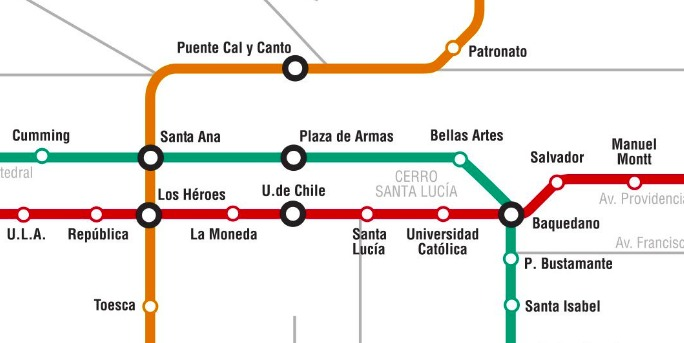
\includegraphics[width=0.9\linewidth]{sec_metro.jpeg}
              \caption{Sección Metro de Santiago, 2010}
              \label{fig:metro}
          \end{figure}
      \end{minipage}
  \end{minipage}
  
 \textbf{Respuesta:}
 
 
    \begin{tikzpicture}[scale=1,transform shape,node distance=1.7cm,main node/.style={circle,draw}]
    
		\node[main node][label = above: \small Puente Cal y Canto][regular polygon, regular polygon sides = 4, draw](1){};
		\node[main node][label = below right: \small Patronato](2)[above right= 0.6cm and 4 cm of 1]{};
		\node[main node][label = above right: Santa Ana](3)[regular polygon, regular polygon sides = 4, draw](3)[below left of = 1]{};
		\node[main node][label = above right: \small Los Héroes][regular polygon, regular polygon sides = 4, draw](4)[below of= 3]{};
		\node[main node][label = left: Toesca](5)[below of = 4]{};
		\node[main node][label = above right: \small Plaza de Armas][regular polygon, regular polygon sides = 4, draw](6)[right = 3 of 3]{};
		\node[main node][label = above right: \small Bellas Artes](7)[right = 3 of 6]{};
		\node[main node][label = above: \small Cumming](8)[left of = 3]{};
		\node[main node][label = below: \small República](9)[left of = 4]{};
		\node[main node][label = below: \small U.L.A](10)[left of = 9]{};
		\node[main node][label = below: \small La Moneda](11)[right of = 4]{};
		\node[main node][label = above: \small U. de Chile][regular polygon, regular polygon sides = 4, draw](12)[right of= 11]{};
		\node[main node][label = below: \small Santa Lucía](13)[right of = 12]{};
		\node[main node][label = below: \small Universidad Católica](14)[right = 3 of 13]{};
		\node[main node][label = below right: \small Baquedano][regular polygon, regular polygon sides = 4, draw](15)[right = 2 of 14]{};
		\node[main node][label = right: \small P.Bustamante](16)[below of = 15]{};
		\node[main node][label = right: \small Santa Isabel](17)[below of = 16]{};
		\node[main node][label = above left: \small Salvador](18)[above right = 1 and 0.5 of 15]{};
		\node[main node][label = above: \small Manuel Montt](19)[right = 0.9 of 18]{};
		\node[main node][scale = 0.01](20) [right = 3 of 1]{};
		\node[main node][scale = 0.01](21) [above = 0.5 of 3]{};
		\node[main node][scale = 0.01](22)[left = 0.5 of 1]{};


		
		\path (8) edge (3);
		\path (3) edge (6);
		\path (6) edge (7);
		\path (7) edge (15);
		\path (14) edge [dashed] (15);
		\path (15) edge [dashed] (18);
		\path (18) edge [dashed] (19);
		\path (10) edge [dashed] (9);
		\path (9) edge [dashed] (4);
		\path (4) edge [dashed] (11);
		\path (11) edge [dashed] (12);
		\path (12) edge [dashed] (13);
		\path (13) edge [dashed] (14);
		\path (15) edge (16);
		\path (16) edge (17);
		\path (3) edge (4);
		\path (4) edge (5);
        \path (3) edge (21);
		\path (21) edge [bend left] (22);
		\path (22) edge (1);
        \path (1) edge (20);
        \path (20) edge [bend right] (2);
		
		
	\end{tikzpicture}
	


\newpage
\item ¡Subamos la complejidad! Utilizando Tikz, agregue el color correspondiente a cada nodo y arco del grafo construido en el ítem anterior. \textbf{Para estaciones comunes utilice \textbf{negro}}. Además, en al menos 3 arcos, indique la distancia en kilómetro que existe entre las estaciones en cuestión (una distancia arbitraria, no es necesario investigar sobre el asunto).

 \textbf{Respuesta:}
 
     \begin{tikzpicture}[scale=1,transform shape,node distance=1.8cm,main node/.style={circle,draw}]
    
		\node[main node][very thick][label = above: \small \textbf{Puente Cal y Canto}][regular polygon, regular polygon sides = 4, draw = black](1){};
		\node[main node][very thick][label = below right: \small Patronato][draw = orange](2)[above right= 0.6cm and 4 cm of 1]{};
		\node[main node][very thick][label = above right: \textbf{Santa Ana}](3)[regular polygon, regular polygon sides = 4, draw](3)[below left of = 1]{};
		\node[main node][very thick][label = above right: \small \textbf{Los Héroes}][regular polygon, regular polygon sides = 4, draw](4)[below of= 3]{};
		\node[main node][very thick][label = left: Toesca][draw = orange](5)[below of = 4]{};
		\node[main node][very thick][label = above right: \small \textbf{Plaza de Armas}][regular polygon, regular polygon sides = 4, draw](6)[right = 3 of 3]{};
		\node[main node][very thick][label = above right: \small Bellas Artes][draw = teal](7)[right = 3 of 6]{};
		\node[main node][very thick][label = above: \small Cumming][draw = teal](8)[left of = 3]{};
		\node[main node][very thick][label = below: \small República][draw = red](9)[left of = 4]{};
		\node[main node][very thick][label = below: \small U.L.A][draw = red](10)[left of = 9]{};
		\node[main node][very thick][label = below: \small La Moneda][draw = red](11)[right of = 4]{};
		\node[main node][very thick][label = above: \small \textbf{U. de Chile}][regular polygon, regular polygon sides = 4, draw](12)[right of= 11]{};
		\node[main node][very thick][label = below: \small Santa Lucía][draw = red](13)[right of = 12]{};
		\node[main node][very thick][label = below: \small Universidad Católica][draw = red](14)[right = 3 of 13]{};
		\node[main node][very thick][label = below right: \small Baquedano][regular polygon, regular polygon sides = 4, draw](15)[right = 2 of 14]{};
		\node[main node][very thick][label = right: \small P.Bustamante][draw = teal](16)[below of = 15]{};
		\node[main node][very thick][label = right: \small Santa Isabel][draw = teal](17)[below of = 16]{};
		\node[main node][very thick][label = above left: \small Salvador][draw = red](18)[above right = 1 and 0.5 of 15]{};
		\node[main node][very thick][label = above: \small Manuel Montt][draw = red](19)[right = 0.9 of 18]{};
		\node[main node][scale = 0.01][draw = orange](20) [right = 3 of 1]{};
		\node[main node][scale = 0.01][draw = orange](21) [above = 0.5 of 3]{};
		\node[main node][scale = 0.01][draw = orange](22)[left = 0.5 of 1]{};


		\path [very thick] (8) edge [draw = teal](3);
		\path [very thick]  (3) edge [draw = teal] (6);
		\path [very thick]  (6) edge  [draw = teal](7);
		\path [very thick] (7) edge  [draw = teal](15);
		\path [very thick]  (14) edge [dashed] [draw = red](15);
		\path [very thick]  (15) edge [dashed] [draw = red](18);
		\path [very thick]  (18) edge [dashed] [draw = red](19);
		\path [very thick] (10) edge [dashed] [draw = red](9);
		\path [very thick] (9) edge [dashed] [draw = red](4);
		\path [very thick] (4) edge [dashed] [draw = red](11);
		\path [very thick] (11) edge [dashed] [draw = red](12);
		\path [very thick] (12) edge [dashed] [draw = red](13);
		\path [very thick] (13) edge [dashed] [draw = red]node [above] {1km}(14);
		\path [very thick] (15) edge  [draw = teal]node [left] {2km}(16);
		\path [very thick] (16) edge  [draw = teal](17) ;
		\path [very thick] (3) edge [draw = orange](4);
		\path [very thick] (4) edge [draw = orange]node [left] {69km}(5);
		\path [very thick] (3) edge [draw = orange] (21);
		\path [very thick](21) edge [draw = orange][bend left] (22);
		\path [very thick](22) edge [draw = orange](1);
        \path [very thick] (1) edge [draw = orange](20);
        \path [very thick] (20) edge [draw = orange][bend right] (2);

		
		
	\end{tikzpicture}
 

\newpage
\item Tikz no solo nos apoyará en la construcción de grafos, sino que podremos escribir algoritmos a través de pseudo--códigos. Un ejemplo (sin sentido) se muestra en el Algoritmo \ref{alg:pri}.

\begin{minipage}{0.35\textwidth}
\begin{algorithm}[H]
\begin{algorithmic}[1]
\STATE{\textbf{procedure} nombre(\(G\))}
\STATE{\(Set<Graph> L\)}
\WHILE{\(len(R) \neq len(V)\)}
	\STATE{\(v = (V-R).pop()\)}
\ENDWHILE
\RETURN{\(L\)}
\end{algorithmic}
\caption{Mi algoritmo}
\label{alg:pri}
\end{algorithm}
\end{minipage}
\hfill
\begin{minipage}{0.6\textwidth}
Escriba dos algoritmos cualquiera (sin sentido si quie\-re) que contengan: \texttt{for, foreach, while, if, else, return}, instrucciones para asignar valores a variables y ope\-raciones. 

\textbf{¡Importante!} Es imperativo que uno de sus algoritmos llame al otro en alguna línea. 
\end{minipage}
\end{enumerate}

\textbf{Respuesta:}

\begin{minipage}{0.4\textwidth}
	
	\begin{algorithm}[H]
		\begin{algorithmic}
			\STATE $lista = [1, 2, 3, 4, 5]$
			\STATE 	\textbf{foreach} $i \textbf{ in } lista$
			\IF {$i\% 2 != 0$} 
				\STATE $lista[i] = i + 1$
			\ELSE
				\STATE $lista[i] = i - 1$
					
			\ENDIF 
			\STATE \textbf{end foreach}
			\STATE $flag = \textbf{true}$
			\WHILE{$i \geq 2$}
				\STATE $lista[i] += 1$
			\ENDWHILE

			\RETURN{$lista$}
			\end{algorithmic}
		
			\caption{Mi algoritmo 1}
	\end{algorithm}
\end{minipage}

\begin{minipage}{0.4\textwidth}
	
	\begin{algorithm}[H]
		\begin{algorithmic}
			\STATE $lista= [1, 2, 3, 4, 5]$
			\STATE $n = 0$
			\STATE $m = lista.\textit{length()}$
			\STATE $listaNueva = []$
			\WHILE{$n \geq m$}
				\STATE $listaNueva = MiAlgoritmo1(lista)$

			\ENDWHILE
		
			\STATE 	\textbf{foreach} $i \textbf{ in } lista$
			\IF {$i != n$} 
				\STATE print(i)
			\ELSE
				\STATE print(i+1)
					
			\ENDIF 
			\STATE \textbf{end foreach}

			\RETURN{$lista$}
			\end{algorithmic}
		
			\caption{Mi algoritmo 2}
	\end{algorithm}
\end{minipage}



%RECUERDE PONER NOMBRE, ROL Y PARALELO EN EL ENCABEZADO

%NO borre lo que sigue porque no compilará
\end{document}



